\documentclass{beamer}  
\usepackage{../slides}
\usepackage{cancel}
%\usepackage{appendixnumberbeamer}
\setbeameroption{hide notes}
\defbeamertemplate{description item}{align left}{\insertdescriptionitem\hfill}




\title[Binary Regressors]{Estimating the Effect of a Mis-measured, Endogenous, Binary Treatment}
\author[FJ DiTraglia]{Francis J.\ DiTraglia\\ Camilo Garcia-Jimeno}
\institute{University of Pennsylvania}
\date{November 19th, 2015}
\begin{document} 
%%%%%%%%%%%%%%%%%%%%%%%%%%%%%%%%%%%%%%%%

\begin{frame}[plain]
	\titlepage 
\end{frame} 
%%%%%%%%%%%%%%%%%%%%%%%%%%%%%%%%%%%%%%%%%
\begin{frame}
  \frametitle{What is the causal effect of $T^*$?}
  \[ y_i = h(T^*_i, \mathbf{x}_i) + \varepsilon_i\]
  \begin{itemize}
    \item $y$ -- Outcome of interest
    \item $h$ -- Unknown function that \emph{does not depend on} $i$
    \item $T^*$ -- Unobserved, endogenous binary treatment
    \item $T$ -- Observed, mis-measured surrogate for $T^*$
    \item $\mathbf{x}$ -- Exogenous covariates
    \item $\varepsilon$ -- Mean-zero error term
    \item $z$ -- Discrete instrumental variable
  \end{itemize}
  %\begin{block}{Target of Inference:}
  %  ATE function:  $\alert{\tau(\mathbf{x}) = h(1,\mathbf{x}) - h(0,\mathbf{x})}$
  %\end{block}
\end{frame}
%%%%%%%%%%%%%%%%%%%%%%%%%%%%%%%%%%%%%%%%%
\begin{frame}
  \frametitle{Example 1: Smoking and Birthweight}
\subtitle{Tappen et al. (2015, BMJ)}
  RCT with 612 pregnant smokers in Glasgow, Scotland: 306 are offered financial incentives to quit smoking.
\begin{itemize}
  \item $y$ -- Birthweight 
  \item $T^*$ -- True smoking behavior 
  \item $T$ -- Self-reported smoking behavior
  \item $\mathbf{x}$ -- Mother characteristics
  \item $z$ -- Offer of financial incentive
\end{itemize}
   
\end{frame}
%%%%%%%%%%%%%%%%%%%%%%%%%%%%%%%%%%%%%%%%%
\begin{frame}
  \frametitle{Example 2: Schooling and Test Scores}
\subtitle{Burde \& Linden (2013, AEJ Applied Economics)}
  RCT in Afghanistan: a school is built in 6 out of 11 villages.
\begin{itemize}
  \item $y$ -- Score on math and language test 
  \item $T^*$ -- True school attendance
  \item $T$ -- Self-reported school attendance
  \item $\mathbf{x}$ -- Household characteristics
  \item $z$ -- School built in village
\end{itemize}
   
\end{frame}
%%%%%%%%%%%%%%%%%%%%%%%%%%%%%%%%%%%%%%%%%
\begin{frame}
  \frametitle{Non-classical Measurement Error: Binary $T^*$}
  \begin{itemize}
    \item Many applications of linear model have \emph{binary} treatment
    \item Binary $T^* \implies \mathbb{E}[T^*w]\leq0$
    \item Misclassification Probabilities:
      \begin{eqnarray*}
        \alpha_0 = \mathbb{P}(T=1|T^*=0)\\
        \alpha_1 = \mathbb{P}(T=0|T^*=1)
      \end{eqnarray*}
    \item Non-Differential Measurement Error: $T\perp (z,u)|T^*$
    \item  $\sigma_{T^*}^2 \nless \sigma_{T}^2$ so work with $\alpha_0, \alpha_1$ rather than $\kappa$ 
    \item \emph{Four-dimensional} Problem\ldots
  \end{itemize}
\end{frame}
%%%%%%%%%%%%%%%%%%%%%%%%%%%%%%%%%%%%%%
\begin{frame}
  \frametitle{Results for a Mis-classified Binary Regressor}
  \begin{block}{Aigner (1973), Bollinger (1996)\ldots}
    \begin{itemize}
      \item Even if $\rho_{T^*u}=0$, OLS is biased and inconsistent: typically attenuated towards zero \emph{but could flip signs!} 
    \end{itemize}
  \end{block}
  \begin{block}{Kane et al.\ (1999), Black et al.\ (2000), Frazis et al.\ (2003)\ldots}
    \begin{itemize}
      \item $\rho_{zu}=0 \implies$ IV solves endogenous regressor problem if there is no mis-classification
      \item $\rho_{T^*u}=0$ and $\rho_{zu}=0 \implies$ non-linear GMM estimator can solve the mis-classification problem
    \end{itemize}
  \end{block}
\end{frame}
%%%%%%%%%%%%%%%%%%%%%%%%%%%%%%%%%%%%%%
\begin{frame}
  \frametitle{OLS and IV Probability Limits: Binary $T^*$}
  \small
  \begin{eqnarray*}
    \mbox{plim}\left(\widehat{\beta}_{OLS} \right) &=& \frac{\sigma_{T^*}^2}{\sigma_T^2}\left[\beta \left( 1 - \alpha_0 - \alpha_1 \right) + \frac{\sigma_{T^*u}}{\sigma_{T^*}^2}\right]\\ \\
    \mbox{plim}\left( \widehat{\beta}_{IV} \right) &=& \frac{\beta}{1 - \alpha_0 - \alpha_1} + \frac{\sigma_{zu}}{\sigma_{zT}}\\ \\ 
    \sigma_{T^*}^2 &=& \frac{\left( p - \alpha_0\right)\left( 1 - p - \alpha_1 \right)}{\left(1 -\alpha_0 - \alpha_1\right)^2}
  \end{eqnarray*}
  Where $p = \mathbb{P}(T=1)$
 
\end{frame}
%%%%%%%%%%%%%%%%%%%%%%%%%%%%%%%%%%%%%%
\begin{frame}
  \frametitle{What About Endogenous, Mis-measured $T^*$, Valid $z$?}
\begin{align*}
 y &= \beta T^* + u\\
u &= c + \varepsilon
\end{align*}

  \begin{itemize}
    \item No results in the literature for this case
    \item Important setting in applied work: e.g.\ RCTs
    \item Discrete Instrument: $z \in \left\{ z_1, \cdots, z_K \right\}$
    \item Non-parametric First Stage: $p_k^* = \mathbb{P}(T^*=1|z = z_k)$
    \item What does $E[\varepsilon|z]=0$ buy us in this case?
  \end{itemize}
\end{frame}
%%%%%%%%%%%%%%%%%%%%%%%%%%%%%%%%%%%%%%
\begin{frame}
  \frametitle{Observable Moments:  $y = \beta T^* + u$}
\begin{center}
  \begin{tabular}{c|c|c|c|c|}
    \multicolumn{1}{c}{}& \multicolumn{1}{c}{$z=1$} &\multicolumn{1}{c}{$z=1$} & \multicolumn{1}{c}{\dots} &\multicolumn{1}{c}{$z=K$}\\
    \cline{2-5}
    $T=0$ & \diagbox[dir=NE]{$\bar{y}_{01}$}{$p_{01}$} & \diagbox[dir=NE]{$\bar{y}_{02}$}{$p_{02}$} & \dots &\diagbox[dir=NE]{$\bar{y}_{0K}$}{$p_{0K}$}\\
    \cline{2-5}
    $T=1$ & \diagbox[dir=NE]{$\bar{y}_{11}$}{$p_{11}$} & \diagbox[dir=NE]{$\bar{y}_{12}$}{$p_{12}$} & \dots &\diagbox[dir=NE]{$\bar{y}_{1K}$}{$p_{1K}$}\\
    \cline{2-5}
  \end{tabular}
\end{center}

\vspace{1em}

\[\bar{y}_{tk} = \mathbb{E}[y|T=t,z=z_k],
\quad p_{tk} =q_k p_k\]
\small
\[q_k = \mathbb{P}(z = z_k), \quad
p_k = \mathbb{P}(T=1|z=z_k)\]
\end{frame}

%%%%%%%%%%%%%%%%%%%%%%%%%%%%%%%%%%%%%%
\begin{frame}
  \frametitle{Unobservable Moments: $y = \beta T^* + u$}
\begin{center}
  \begin{tabular}{c|c|c|c|c|}
    \multicolumn{1}{c}{}& \multicolumn{1}{c}{$z=1$} &\multicolumn{1}{c}{$z=1$} & \multicolumn{1}{c}{\dots} &\multicolumn{1}{c}{$z=K$}\\
    \cline{2-5}
    $T^*=0$ & \diagbox[dir=NE]{$m^*_{01}$}{$p^*_{01}$} & \diagbox[dir=NE]{$m^*_{02}$}{$p^*_{02}$} & \dots &\diagbox[dir=NE]{$m^*_{0K}$}{$p^*_{0K}$}\\
    \cline{2-5}
    $T^*=1$ & \diagbox[dir=NE]{$m^*_{11}$}{$p^*_{11}$} & \diagbox[dir=NE]{$m^*_{12}$}{$p^*_{12}$} & \dots &\diagbox[dir=NE]{$m^*_{1K}$}{$p^*_{1K}$}\\
    \cline{2-5}
  \end{tabular}
\end{center}

\vspace{1em}

\[m^*_{tk} = \mathbb{E}[u|T^*=t,z=z_k],
\quad p^*_{tk}=q_k p^*_k\]
\small
\[p^*_k=\mathbb{P}(T^*=1|z=z_k) = \frac{p_k - \alpha_0}{1 - \alpha_0 - \alpha_1} \]
\end{frame}
%%%%%%%%%%%%%%%%%%%%%%%%%%%%%%%%%%%%%%
\begin{frame}
  \frametitle{Possible Assumptions On $m^*_{tk}$}
  \begin{block}{Joint Exogeneity: $\mathbb{E}[\varepsilon|T^*,z]=0$}
    $\implies m^*_{tk} =c \quad$ for all $t,k$
  \end{block}
  \begin{block}{Exogenous Treatment: $\mathbb{E}[\varepsilon|T^*]=0$}
    $\implies \displaystyle \frac{1}{\mathbb{P}(T^*=t)}\sum_{k}p^*_{tk}m^*_{tk} = c\quad$  for all $t$
  \end{block}
  \begin{alertblock}{Exogenous Instrument: $\mathbb{E}[\varepsilon|z]=0$}
    $\implies (1-p^*_k)m^*_{0k} + p^*_k m^*_{1k}=c \quad$ for all $k$
  \end{alertblock}
\end{frame}
%%%%%%%%%%%%%%%%%%%%%%%%%%%%%%%%%%%%%%
\begin{frame}
  \frametitle{Moment Conditions Imposing $\mathbb{E}[\varepsilon|z]=0$}
  One pair of equations for each $k = 1, \dots, K$
\begin{align*}
  \hat{y}_{0k} &=\alpha_1(p_k - \alpha_0)\left(\frac{\beta}{1 - \alpha_0 - \alpha_1}\right) + (1-\alpha_0)c - (p _k -  \alpha_0)m_{1k}^* \\[1.5ex]
  \label{eq:MC1IV}
  \hat{y}_{1k} &=(1-\alpha_1)(p_k - \alpha_0)\left(\frac{\beta}{1 - \alpha_0 - \alpha_1}\right) + \alpha_0 c + (p _k -  \alpha_0)m_{1k}^*
\end{align*}

\vspace{0.5em}
where $\hat{y}_{0k}=(1-p_k)\bar{y}_{0k}$ and $\hat{y}_{0k}=p_k\bar{y}_{1k}$


\vspace{2em} 

\hfill \alert{\framebox{$2K$ Equations in $K+4$ Unknowns}}
\end{frame}
%%%%%%%%%%%%%%%%%%%%%%%%%%%%%%%%%%%%%%
\begin{frame}
  \frametitle{Mahajan}
\end{frame}
%%%%%%%%%%%%%%%%%%%%%%%%%%%%%%%%%%%%%%
\begin{frame}
  \frametitle{\emph{Proposition}: $\beta$ is Undentified Regardless of $K$}
  \begin{block}{Proof Sketch}
    \begin{enumerate}[(1)]
      \item Show that $\mathcal{W}= \beta/(1-\alpha_0 - \alpha_1)$ is identified. 
      \item Show that $\mathcal{Q} = c + \beta(1-\alpha_0)/(1-\alpha_0-\alpha_1)$ is identified.
      \item $(1) + (2) \implies (\mathcal{Q}, \mathcal{W})$ are \emph{fixed}
      \item Use (3) to rewrite equations in terms of $(\mathcal{Q}, \mathcal{W})$.
      \item Discover that there is only \emph{one} equation per $k$! Rearranging: 

        \[m^*_{1k} = \frac{\mathcal{W}(\hat{y}_{0k}-\alpha_1 \mathcal{Q}) - \beta(\mathcal{Q}-\beta-\mathcal{W}\alpha_1) + \mathcal{W}^2(1-p_k)\alpha_1}{\mathcal{W}(1-p_k - \alpha_1) - \beta}\]
    \end{enumerate}

  \end{block} 
    
\end{frame}
%%%%%%%%%%%%%%%%%%%%%%%%%%%%%%%%%%%%%%
\begin{frame}
  \frametitle{Special Case of Prev Proof: $\alpha_0 = 0$}
\begin{align*}
  \hat{y}_{0k} &=c + p_k \beta \left(\frac{\alpha_1}{1 -  \alpha_1}\right) - p _k m_{1k}^* \\[1.5ex]
  \hat{y}_{1k} &=p_k \beta + p _k m_{1k}^*
\end{align*}
\end{frame}
%%%%%%%%%%%%%%%%%%%%%%%%%%%%%%%%%%%%%%
\begin{frame}
  \frametitle{Identification by Conditional Variances?} 
  \begin{block}{New Assumption}
    Homoskedastic errors w.r.t.\ the \emph{instrument}: $E[\varepsilon^2|z]=E[\varepsilon^2]$
  \end{block}
  \begin{block}{Not Crazy!}
    Holds in an RCT or a \emph{true} natural experiment.
  \end{block}
  \begin{alertblock}{New Moment Conditions}
    For each pair $(k,\ell)$
\begin{align*}
  s^2_k - s^2_\ell = \mathcal{W}^2\left[p_k(1-p_k) - p_\ell(1-p_\ell) + (\alpha_0 - \alpha_1)(p_k - p_\ell)\right]\\  
  + 2\mathcal{W}\left[(p_k - \alpha_0)(m^*_{1k}-c) - (p_\ell - \alpha_0)(m^*_{1\ell}-c)\right]
\end{align*}

\vspace{0.5em}
Where $s^2_k = Var(y|z=z_k)$, and $\mathcal{W}$ is the Wald IV estimator. 
  \end{alertblock}
\end{frame}
%%%%%%%%%%%%%%%%%%%%%%%%%%%%%%%%%%%%%%
\begin{frame}
  \frametitle{\emph{Proposition}: $(\alpha_0 - \alpha_1)$ is Identified}
  Define
\begin{equation*}
  \widetilde{\mathcal{W}}_{k\ell} = \frac{\mathbb{E}[yT|z_k] - \mathbb{E}[yT|z_\ell]}{p_k - p_\ell}
\end{equation*}
Show that:
\begin{align*}
(p_k - \alpha_0)&(m^*_{1k}-c) - (p_\ell - \alpha_0)(m^*_{1\ell}-c) =\\
& (p_k - p_\ell)\left[ \widetilde{W}_{k\ell} - \mathbb{E}[y] - \mathcal{W}\left\{ (1 - p) + (\alpha_0 - \alpha_1) \right\} \right]
\end{align*}
Substituting and rearranging: 
\begin{equation*}
  \alpha_0 - \alpha_1 = (2p - 1 - p_k - p_\ell) + \frac{2(\widetilde{W}_{k\ell} - \mathbb{E}[y])}{\mathcal{W}} - \frac{s_k^2 - s_\ell^2}{(p_k - p_\ell)\mathcal{W}^2}
\end{equation*}
\end{frame}
%%%%%%%%%%%%%%%%%%%%%%%%%%%%%%%%%%%%%%
\begin{frame}
  \frametitle{What Good is $(\alpha_0 - \alpha_1)?$}
    \begin{itemize}
      \item Test a necessary condition for \emph{no mis-classification}:$\alpha_0 = \alpha_1$ 
      \item Simple, tighter partial identification bounds for $\beta$
      \item In some settings, one of the mis-classification probabilities is known to be zero $\implies \beta$ point identified 
    \end{itemize}
\end{frame}
%%%%%%%%%%%%%%%%%%%%%%%%%%%%%%%%%%%%%%
\begin{frame}
  \frametitle{Identification from Third Moments}
\end{frame}
%%%%%%%%%%%%%%%%%%%%%%%%%%%%%%%%%%%%%%
\begin{frame}
  \frametitle{Simulation Study}
  $y = \beta T^* + \varepsilon$

  $T^* = \mathbf{1}\left\{ \gamma_0 + \gamma_1 z + \eta > 0 \right\}$

  $\gamma_0 = \Phi^{-1}(\delta)$, $\gamma_1 = \Phi^{-1}(1-\delta) - \Phi(\delta)$ so that $\delta$

  E.g.\ if $\delta=0.1$ then 10\% of those \emph{not} offered treatment get it anyway, and 10\% of those offered treatment don't take it up.
  
  If $T^*=0$ then $T=0$ (E.g.\ Birthweight and smoking)
  $T|T^*=1 \sim \mbox{Bernoulli}(?)$

  \[ \left[
  \begin{array}{c}
  \varepsilon \\ \eta
\end{array}
\right] \sim N\left( \left[
\begin{array}{c}
0 \\ 0
\end{array}
\right], \left[
\begin{array}{cc}
1 & 0.3\\
0.3 & 1 \\
\end{array}
\right]\right)\]
\end{frame}
%%%%%%%%%%%%%%%%%%%%%%%%%%%%%%%%%%%%%%
\begin{frame}

\begin{figure}[h]
  \scriptsize

  \begingroup
  \tikzset{every picture/.style={scale=0.58}}%
  \centering
  \begin{subfigure}[b]{0.48\textwidth}
  % Created by tikzDevice version 0.8.1 on 2015-11-15 17:38:49
% !TEX encoding = UTF-8 Unicode
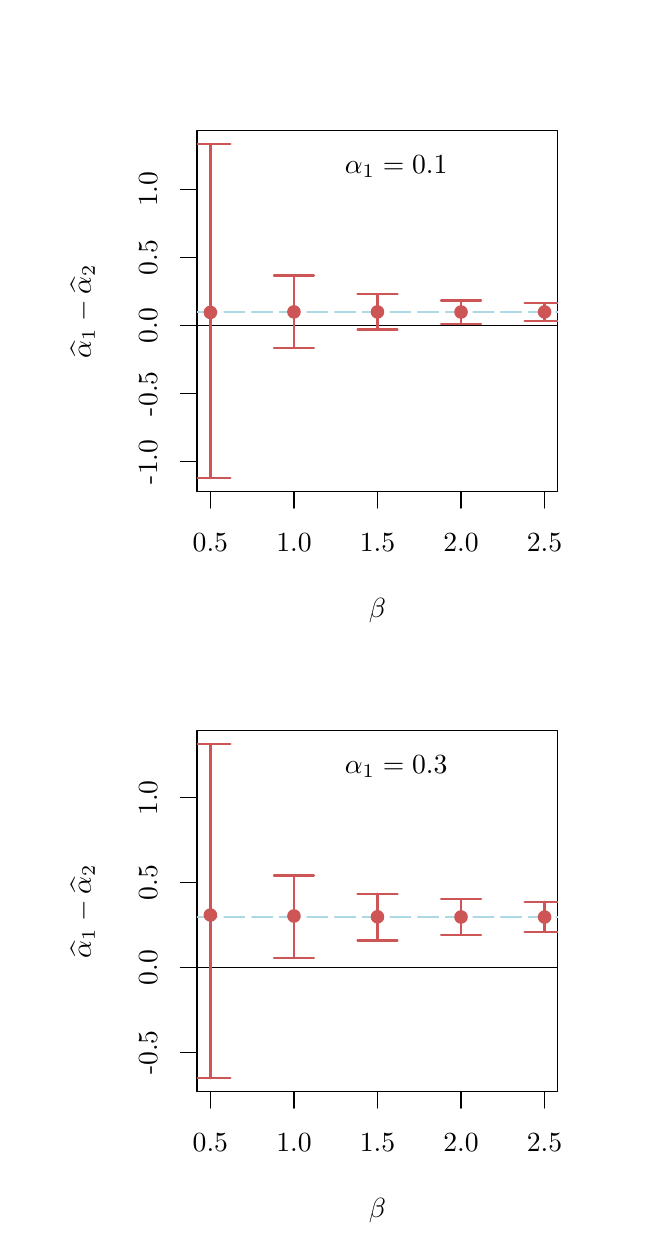
\begin{tikzpicture}[x=1pt,y=1pt]
\definecolor{fillColor}{RGB}{255,255,255}
\path[use as bounding box,fill=fillColor,fill opacity=0.00] (0,0) rectangle (216.81,433.62);
\begin{scope}
\path[clip] ( 61.20,266.01) rectangle (191.61,396.42);
\definecolor{drawColor}{RGB}{255,255,255}
\definecolor{fillColor}{RGB}{255,255,255}

\path[draw=drawColor,line width= 0.4pt,line join=round,line cap=round,fill=fillColor] ( 66.03,330.73) circle (  2.25);

\path[draw=drawColor,line width= 0.4pt,line join=round,line cap=round,fill=fillColor] ( 96.22,330.91) circle (  2.25);

\path[draw=drawColor,line width= 0.4pt,line join=round,line cap=round,fill=fillColor] (126.40,330.90) circle (  2.25);

\path[draw=drawColor,line width= 0.4pt,line join=round,line cap=round,fill=fillColor] (156.59,330.87) circle (  2.25);

\path[draw=drawColor,line width= 0.4pt,line join=round,line cap=round,fill=fillColor] (186.78,330.89) circle (  2.25);
\end{scope}
\begin{scope}
\path[clip] (  0.00,  0.00) rectangle (216.81,433.62);
\definecolor{drawColor}{RGB}{0,0,0}

\path[draw=drawColor,line width= 0.4pt,line join=round,line cap=round] ( 66.03,266.01) -- (186.78,266.01);

\path[draw=drawColor,line width= 0.4pt,line join=round,line cap=round] ( 66.03,266.01) -- ( 66.03,260.01);

\path[draw=drawColor,line width= 0.4pt,line join=round,line cap=round] ( 96.22,266.01) -- ( 96.22,260.01);

\path[draw=drawColor,line width= 0.4pt,line join=round,line cap=round] (126.40,266.01) -- (126.40,260.01);

\path[draw=drawColor,line width= 0.4pt,line join=round,line cap=round] (156.59,266.01) -- (156.59,260.01);

\path[draw=drawColor,line width= 0.4pt,line join=round,line cap=round] (186.78,266.01) -- (186.78,260.01);

\node[text=drawColor,anchor=base,inner sep=0pt, outer sep=0pt, scale=  1.00] at ( 66.03,244.41) {0.5};

\node[text=drawColor,anchor=base,inner sep=0pt, outer sep=0pt, scale=  1.00] at ( 96.22,244.41) {1.0};

\node[text=drawColor,anchor=base,inner sep=0pt, outer sep=0pt, scale=  1.00] at (126.40,244.41) {1.5};

\node[text=drawColor,anchor=base,inner sep=0pt, outer sep=0pt, scale=  1.00] at (156.59,244.41) {2.0};

\node[text=drawColor,anchor=base,inner sep=0pt, outer sep=0pt, scale=  1.00] at (186.78,244.41) {2.5};

\path[draw=drawColor,line width= 0.4pt,line join=round,line cap=round] ( 61.20,276.72) -- ( 61.20,375.22);

\path[draw=drawColor,line width= 0.4pt,line join=round,line cap=round] ( 61.20,276.72) -- ( 55.20,276.72);

\path[draw=drawColor,line width= 0.4pt,line join=round,line cap=round] ( 61.20,301.34) -- ( 55.20,301.34);

\path[draw=drawColor,line width= 0.4pt,line join=round,line cap=round] ( 61.20,325.97) -- ( 55.20,325.97);

\path[draw=drawColor,line width= 0.4pt,line join=round,line cap=round] ( 61.20,350.59) -- ( 55.20,350.59);

\path[draw=drawColor,line width= 0.4pt,line join=round,line cap=round] ( 61.20,375.22) -- ( 55.20,375.22);

\node[text=drawColor,rotate= 90.00,anchor=base,inner sep=0pt, outer sep=0pt, scale=  1.00] at ( 46.80,276.72) {-1.0};

\node[text=drawColor,rotate= 90.00,anchor=base,inner sep=0pt, outer sep=0pt, scale=  1.00] at ( 46.80,301.34) {-0.5};

\node[text=drawColor,rotate= 90.00,anchor=base,inner sep=0pt, outer sep=0pt, scale=  1.00] at ( 46.80,325.97) {0.0};

\node[text=drawColor,rotate= 90.00,anchor=base,inner sep=0pt, outer sep=0pt, scale=  1.00] at ( 46.80,350.59) {0.5};

\node[text=drawColor,rotate= 90.00,anchor=base,inner sep=0pt, outer sep=0pt, scale=  1.00] at ( 46.80,375.22) {1.0};

\path[draw=drawColor,line width= 0.4pt,line join=round,line cap=round] ( 61.20,266.01) --
	(191.61,266.01) --
	(191.61,396.42) --
	( 61.20,396.42) --
	( 61.20,266.01);
\end{scope}
\begin{scope}
\path[clip] (  0.00,216.81) rectangle (216.81,433.62);
\definecolor{drawColor}{RGB}{0,0,0}

\node[text=drawColor,anchor=base,inner sep=0pt, outer sep=0pt, scale=  1.00] at (126.41,220.41) {$\beta$};

\node[text=drawColor,rotate= 90.00,anchor=base,inner sep=0pt, outer sep=0pt, scale=  1.00] at ( 22.80,331.22) {$\widehat{\alpha}_1 - \widehat{\alpha}_2$};
\end{scope}
\begin{scope}
\path[clip] ( 61.20,266.01) rectangle (191.61,396.42);
\definecolor{drawColor}{RGB}{0,0,0}

\node[text=drawColor,anchor=base west,inner sep=0pt, outer sep=0pt, scale=  1.00] at (114.66,380.98) {$\alpha_1=0.1$};
\definecolor{drawColor}{RGB}{173,216,230}

\path[draw=drawColor,line width= 0.8pt,dash pattern=on 7pt off 3pt ,line join=round,line cap=round] ( 61.20,330.89) -- (191.61,330.89);

\path[draw=drawColor,line width= 0.8pt,dash pattern=on 7pt off 3pt ,line join=round,line cap=round] ( 61.20,330.89) -- (191.61,330.89);

\path[draw=drawColor,line width= 0.8pt,dash pattern=on 7pt off 3pt ,line join=round,line cap=round] ( 61.20,330.89) -- (191.61,330.89);

\path[draw=drawColor,line width= 0.8pt,dash pattern=on 7pt off 3pt ,line join=round,line cap=round] ( 61.20,330.89) -- (191.61,330.89);

\path[draw=drawColor,line width= 0.8pt,dash pattern=on 7pt off 3pt ,line join=round,line cap=round] ( 61.20,330.89) -- (191.61,330.89);
\definecolor{drawColor}{RGB}{0,0,0}

\path[draw=drawColor,line width= 0.4pt,line join=round,line cap=round] ( 61.20,325.97) -- (191.61,325.97);
\definecolor{drawColor}{RGB}{205,85,85}

\path[draw=drawColor,line width= 0.8pt,line join=round,line cap=round] ( 66.03,270.84) -- ( 66.03,391.59);

\path[draw=drawColor,line width= 0.8pt,line join=round,line cap=round] ( 58.80,270.84) --
	( 66.03,270.84) --
	( 73.26,270.84);

\path[draw=drawColor,line width= 0.8pt,line join=round,line cap=round] ( 73.26,391.59) --
	( 66.03,391.59) --
	( 58.80,391.59);

\path[draw=drawColor,line width= 0.8pt,line join=round,line cap=round] ( 96.22,317.85) -- ( 96.22,344.08);

\path[draw=drawColor,line width= 0.8pt,line join=round,line cap=round] ( 88.99,317.85) --
	( 96.22,317.85) --
	(103.44,317.85);

\path[draw=drawColor,line width= 0.8pt,line join=round,line cap=round] (103.44,344.08) --
	( 96.22,344.08) --
	( 88.99,344.08);

\path[draw=drawColor,line width= 0.8pt,line join=round,line cap=round] (126.40,324.52) -- (126.40,337.30);

\path[draw=drawColor,line width= 0.8pt,line join=round,line cap=round] (119.18,324.52) --
	(126.40,324.52) --
	(133.63,324.52);

\path[draw=drawColor,line width= 0.8pt,line join=round,line cap=round] (133.63,337.30) --
	(126.40,337.30) --
	(119.18,337.30);

\path[draw=drawColor,line width= 0.8pt,line join=round,line cap=round] (156.59,326.65) -- (156.59,335.06);

\path[draw=drawColor,line width= 0.8pt,line join=round,line cap=round] (149.37,326.65) --
	(156.59,326.65) --
	(163.82,326.65);

\path[draw=drawColor,line width= 0.8pt,line join=round,line cap=round] (163.82,335.06) --
	(156.59,335.06) --
	(149.37,335.06);

\path[draw=drawColor,line width= 0.8pt,line join=round,line cap=round] (186.78,327.61) -- (186.78,334.14);

\path[draw=drawColor,line width= 0.8pt,line join=round,line cap=round] (179.55,327.61) --
	(186.78,327.61) --
	(194.01,327.61);

\path[draw=drawColor,line width= 0.8pt,line join=round,line cap=round] (194.01,334.14) --
	(186.78,334.14) --
	(179.55,334.14);
\definecolor{fillColor}{RGB}{205,85,85}

\path[draw=drawColor,line width= 0.4pt,line join=round,line cap=round,fill=fillColor] ( 66.03,330.73) circle (  2.25);

\path[draw=drawColor,line width= 0.4pt,line join=round,line cap=round,fill=fillColor] ( 96.22,330.91) circle (  2.25);

\path[draw=drawColor,line width= 0.4pt,line join=round,line cap=round,fill=fillColor] (126.40,330.90) circle (  2.25);

\path[draw=drawColor,line width= 0.4pt,line join=round,line cap=round,fill=fillColor] (156.59,330.87) circle (  2.25);

\path[draw=drawColor,line width= 0.4pt,line join=round,line cap=round,fill=fillColor] (186.78,330.89) circle (  2.25);
\end{scope}
\begin{scope}
\path[clip] ( 61.20, 49.20) rectangle (191.61,179.61);
\definecolor{drawColor}{RGB}{255,255,255}
\definecolor{fillColor}{RGB}{255,255,255}

\path[draw=drawColor,line width= 0.4pt,line join=round,line cap=round,fill=fillColor] ( 66.03,112.98) circle (  2.25);

\path[draw=drawColor,line width= 0.4pt,line join=round,line cap=round,fill=fillColor] ( 96.22,112.62) circle (  2.25);

\path[draw=drawColor,line width= 0.4pt,line join=round,line cap=round,fill=fillColor] (126.40,112.33) circle (  2.25);

\path[draw=drawColor,line width= 0.4pt,line join=round,line cap=round,fill=fillColor] (156.59,112.27) circle (  2.25);

\path[draw=drawColor,line width= 0.4pt,line join=round,line cap=round,fill=fillColor] (186.78,112.24) circle (  2.25);
\end{scope}
\begin{scope}
\path[clip] (  0.00,  0.00) rectangle (216.81,433.62);
\definecolor{drawColor}{RGB}{0,0,0}

\path[draw=drawColor,line width= 0.4pt,line join=round,line cap=round] ( 66.03, 49.20) -- (186.78, 49.20);

\path[draw=drawColor,line width= 0.4pt,line join=round,line cap=round] ( 66.03, 49.20) -- ( 66.03, 43.20);

\path[draw=drawColor,line width= 0.4pt,line join=round,line cap=round] ( 96.22, 49.20) -- ( 96.22, 43.20);

\path[draw=drawColor,line width= 0.4pt,line join=round,line cap=round] (126.40, 49.20) -- (126.40, 43.20);

\path[draw=drawColor,line width= 0.4pt,line join=round,line cap=round] (156.59, 49.20) -- (156.59, 43.20);

\path[draw=drawColor,line width= 0.4pt,line join=round,line cap=round] (186.78, 49.20) -- (186.78, 43.20);

\node[text=drawColor,anchor=base,inner sep=0pt, outer sep=0pt, scale=  1.00] at ( 66.03, 27.60) {0.5};

\node[text=drawColor,anchor=base,inner sep=0pt, outer sep=0pt, scale=  1.00] at ( 96.22, 27.60) {1.0};

\node[text=drawColor,anchor=base,inner sep=0pt, outer sep=0pt, scale=  1.00] at (126.40, 27.60) {1.5};

\node[text=drawColor,anchor=base,inner sep=0pt, outer sep=0pt, scale=  1.00] at (156.59, 27.60) {2.0};

\node[text=drawColor,anchor=base,inner sep=0pt, outer sep=0pt, scale=  1.00] at (186.78, 27.60) {2.5};

\path[draw=drawColor,line width= 0.4pt,line join=round,line cap=round] ( 61.20, 63.24) -- ( 61.20,155.30);

\path[draw=drawColor,line width= 0.4pt,line join=round,line cap=round] ( 61.20, 63.24) -- ( 55.20, 63.24);

\path[draw=drawColor,line width= 0.4pt,line join=round,line cap=round] ( 61.20, 93.93) -- ( 55.20, 93.93);

\path[draw=drawColor,line width= 0.4pt,line join=round,line cap=round] ( 61.20,124.62) -- ( 55.20,124.62);

\path[draw=drawColor,line width= 0.4pt,line join=round,line cap=round] ( 61.20,155.30) -- ( 55.20,155.30);

\node[text=drawColor,rotate= 90.00,anchor=base,inner sep=0pt, outer sep=0pt, scale=  1.00] at ( 46.80, 63.24) {-0.5};

\node[text=drawColor,rotate= 90.00,anchor=base,inner sep=0pt, outer sep=0pt, scale=  1.00] at ( 46.80, 93.93) {0.0};

\node[text=drawColor,rotate= 90.00,anchor=base,inner sep=0pt, outer sep=0pt, scale=  1.00] at ( 46.80,124.62) {0.5};

\node[text=drawColor,rotate= 90.00,anchor=base,inner sep=0pt, outer sep=0pt, scale=  1.00] at ( 46.80,155.30) {1.0};

\path[draw=drawColor,line width= 0.4pt,line join=round,line cap=round] ( 61.20, 49.20) --
	(191.61, 49.20) --
	(191.61,179.61) --
	( 61.20,179.61) --
	( 61.20, 49.20);
\end{scope}
\begin{scope}
\path[clip] (  0.00,  0.00) rectangle (216.81,216.81);
\definecolor{drawColor}{RGB}{0,0,0}

\node[text=drawColor,anchor=base,inner sep=0pt, outer sep=0pt, scale=  1.00] at (126.41,  3.60) {$\beta$};

\node[text=drawColor,rotate= 90.00,anchor=base,inner sep=0pt, outer sep=0pt, scale=  1.00] at ( 22.80,114.41) {$\widehat{\alpha}_1 - \widehat{\alpha}_2$};
\end{scope}
\begin{scope}
\path[clip] ( 61.20, 49.20) rectangle (191.61,179.61);
\definecolor{drawColor}{RGB}{0,0,0}

\node[text=drawColor,anchor=base west,inner sep=0pt, outer sep=0pt, scale=  1.00] at (114.66,164.17) {$\alpha_1=0.3$};
\definecolor{drawColor}{RGB}{173,216,230}

\path[draw=drawColor,line width= 0.8pt,dash pattern=on 7pt off 3pt ,line join=round,line cap=round] ( 61.20,112.34) -- (191.61,112.34);

\path[draw=drawColor,line width= 0.8pt,dash pattern=on 7pt off 3pt ,line join=round,line cap=round] ( 61.20,112.34) -- (191.61,112.34);

\path[draw=drawColor,line width= 0.8pt,dash pattern=on 7pt off 3pt ,line join=round,line cap=round] ( 61.20,112.34) -- (191.61,112.34);

\path[draw=drawColor,line width= 0.8pt,dash pattern=on 7pt off 3pt ,line join=round,line cap=round] ( 61.20,112.34) -- (191.61,112.34);

\path[draw=drawColor,line width= 0.8pt,dash pattern=on 7pt off 3pt ,line join=round,line cap=round] ( 61.20,112.34) -- (191.61,112.34);
\definecolor{drawColor}{RGB}{0,0,0}

\path[draw=drawColor,line width= 0.4pt,line join=round,line cap=round] ( 61.20, 93.93) -- (191.61, 93.93);
\definecolor{drawColor}{RGB}{205,85,85}

\path[draw=drawColor,line width= 0.8pt,line join=round,line cap=round] ( 66.03, 54.03) -- ( 66.03,174.78);

\path[draw=drawColor,line width= 0.8pt,line join=round,line cap=round] ( 58.80, 54.03) --
	( 66.03, 54.03) --
	( 73.26, 54.03);

\path[draw=drawColor,line width= 0.8pt,line join=round,line cap=round] ( 73.26,174.78) --
	( 66.03,174.78) --
	( 58.80,174.78);

\path[draw=drawColor,line width= 0.8pt,line join=round,line cap=round] ( 96.22, 97.35) -- ( 96.22,127.29);

\path[draw=drawColor,line width= 0.8pt,line join=round,line cap=round] ( 88.99, 97.35) --
	( 96.22, 97.35) --
	(103.44, 97.35);

\path[draw=drawColor,line width= 0.8pt,line join=round,line cap=round] (103.44,127.29) --
	( 96.22,127.29) --
	( 88.99,127.29);

\path[draw=drawColor,line width= 0.8pt,line join=round,line cap=round] (126.40,103.73) -- (126.40,120.66);

\path[draw=drawColor,line width= 0.8pt,line join=round,line cap=round] (119.18,103.73) --
	(126.40,103.73) --
	(133.63,103.73);

\path[draw=drawColor,line width= 0.8pt,line join=round,line cap=round] (133.63,120.66) --
	(126.40,120.66) --
	(119.18,120.66);

\path[draw=drawColor,line width= 0.8pt,line join=round,line cap=round] (156.59,105.89) -- (156.59,118.72);

\path[draw=drawColor,line width= 0.8pt,line join=round,line cap=round] (149.37,105.89) --
	(156.59,105.89) --
	(163.82,105.89);

\path[draw=drawColor,line width= 0.8pt,line join=round,line cap=round] (163.82,118.72) --
	(156.59,118.72) --
	(149.37,118.72);

\path[draw=drawColor,line width= 0.8pt,line join=round,line cap=round] (186.78,106.93) -- (186.78,117.79);

\path[draw=drawColor,line width= 0.8pt,line join=round,line cap=round] (179.55,106.93) --
	(186.78,106.93) --
	(194.01,106.93);

\path[draw=drawColor,line width= 0.8pt,line join=round,line cap=round] (194.01,117.79) --
	(186.78,117.79) --
	(179.55,117.79);
\definecolor{fillColor}{RGB}{205,85,85}

\path[draw=drawColor,line width= 0.4pt,line join=round,line cap=round,fill=fillColor] ( 66.03,112.98) circle (  2.25);

\path[draw=drawColor,line width= 0.4pt,line join=round,line cap=round,fill=fillColor] ( 96.22,112.62) circle (  2.25);

\path[draw=drawColor,line width= 0.4pt,line join=round,line cap=round,fill=fillColor] (126.40,112.33) circle (  2.25);

\path[draw=drawColor,line width= 0.4pt,line join=round,line cap=round,fill=fillColor] (156.59,112.27) circle (  2.25);

\path[draw=drawColor,line width= 0.4pt,line join=round,line cap=round,fill=fillColor] (186.78,112.24) circle (  2.25);
\end{scope}
\end{tikzpicture}

%\caption{Caption here!}
\label{fig:a_test}
  \end{subfigure}
  ~
  \begin{subfigure}[b]{0.48\textwidth}
  % Created by tikzDevice version 0.8.1 on 2015-11-15 18:06:45
% !TEX encoding = UTF-8 Unicode
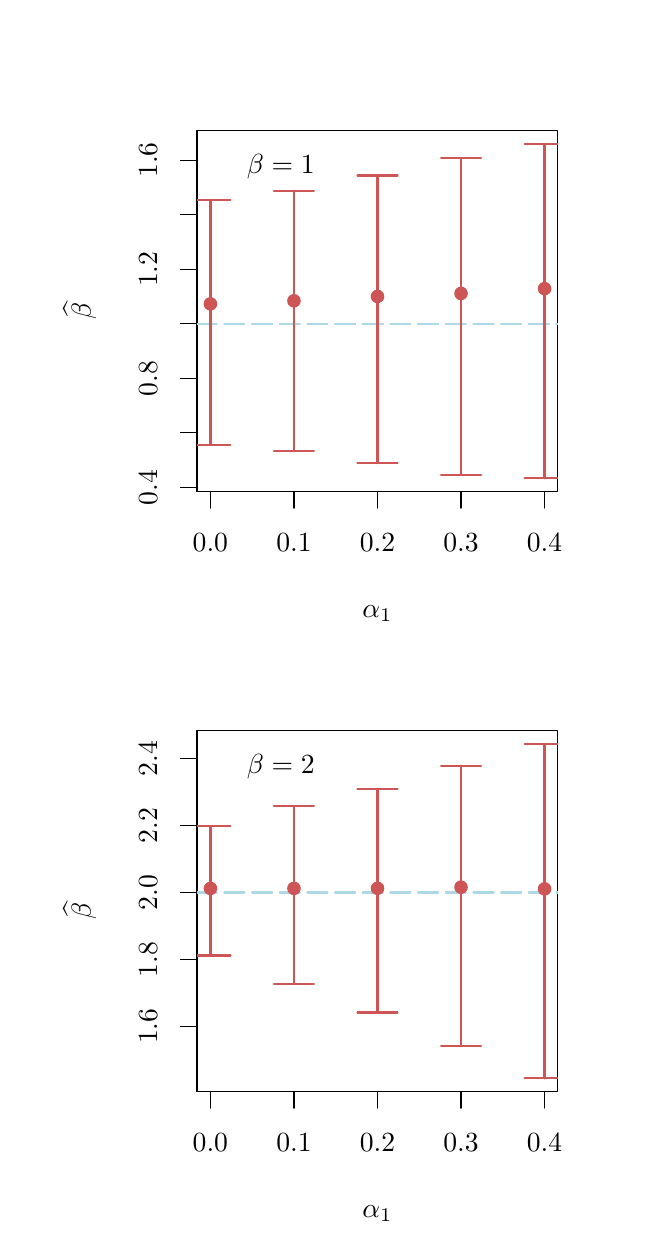
\begin{tikzpicture}[x=1pt,y=1pt]
\definecolor{fillColor}{RGB}{255,255,255}
\path[use as bounding box,fill=fillColor,fill opacity=0.00] (0,0) rectangle (216.81,433.62);
\begin{scope}
\path[clip] ( 61.20,266.01) rectangle (191.61,396.42);
\definecolor{drawColor}{RGB}{255,255,255}
\definecolor{fillColor}{RGB}{255,255,255}

\path[draw=drawColor,line width= 0.4pt,line join=round,line cap=round,fill=fillColor] ( 66.03,333.81) circle (  2.25);

\path[draw=drawColor,line width= 0.4pt,line join=round,line cap=round,fill=fillColor] ( 96.22,334.92) circle (  2.25);

\path[draw=drawColor,line width= 0.4pt,line join=round,line cap=round,fill=fillColor] (126.41,336.50) circle (  2.25);

\path[draw=drawColor,line width= 0.4pt,line join=round,line cap=round,fill=fillColor] (156.59,337.58) circle (  2.25);

\path[draw=drawColor,line width= 0.4pt,line join=round,line cap=round,fill=fillColor] (186.78,339.31) circle (  2.25);
\end{scope}
\begin{scope}
\path[clip] (  0.00,  0.00) rectangle (216.81,433.62);
\definecolor{drawColor}{RGB}{0,0,0}

\path[draw=drawColor,line width= 0.4pt,line join=round,line cap=round] ( 66.03,266.01) -- (186.78,266.01);

\path[draw=drawColor,line width= 0.4pt,line join=round,line cap=round] ( 66.03,266.01) -- ( 66.03,260.01);

\path[draw=drawColor,line width= 0.4pt,line join=round,line cap=round] ( 96.22,266.01) -- ( 96.22,260.01);

\path[draw=drawColor,line width= 0.4pt,line join=round,line cap=round] (126.41,266.01) -- (126.41,260.01);

\path[draw=drawColor,line width= 0.4pt,line join=round,line cap=round] (156.59,266.01) -- (156.59,260.01);

\path[draw=drawColor,line width= 0.4pt,line join=round,line cap=round] (186.78,266.01) -- (186.78,260.01);

\node[text=drawColor,anchor=base,inner sep=0pt, outer sep=0pt, scale=  1.00] at ( 66.03,244.41) {0.0};

\node[text=drawColor,anchor=base,inner sep=0pt, outer sep=0pt, scale=  1.00] at ( 96.22,244.41) {0.1};

\node[text=drawColor,anchor=base,inner sep=0pt, outer sep=0pt, scale=  1.00] at (126.41,244.41) {0.2};

\node[text=drawColor,anchor=base,inner sep=0pt, outer sep=0pt, scale=  1.00] at (156.59,244.41) {0.3};

\node[text=drawColor,anchor=base,inner sep=0pt, outer sep=0pt, scale=  1.00] at (186.78,244.41) {0.4};

\path[draw=drawColor,line width= 0.4pt,line join=round,line cap=round] ( 61.20,267.47) -- ( 61.20,385.77);

\path[draw=drawColor,line width= 0.4pt,line join=round,line cap=round] ( 61.20,267.47) -- ( 55.20,267.47);

\path[draw=drawColor,line width= 0.4pt,line join=round,line cap=round] ( 61.20,287.18) -- ( 55.20,287.18);

\path[draw=drawColor,line width= 0.4pt,line join=round,line cap=round] ( 61.20,306.90) -- ( 55.20,306.90);

\path[draw=drawColor,line width= 0.4pt,line join=round,line cap=round] ( 61.20,326.62) -- ( 55.20,326.62);

\path[draw=drawColor,line width= 0.4pt,line join=round,line cap=round] ( 61.20,346.33) -- ( 55.20,346.33);

\path[draw=drawColor,line width= 0.4pt,line join=round,line cap=round] ( 61.20,366.05) -- ( 55.20,366.05);

\path[draw=drawColor,line width= 0.4pt,line join=round,line cap=round] ( 61.20,385.77) -- ( 55.20,385.77);

\node[text=drawColor,rotate= 90.00,anchor=base,inner sep=0pt, outer sep=0pt, scale=  1.00] at ( 46.80,267.47) {0.4};

\node[text=drawColor,rotate= 90.00,anchor=base,inner sep=0pt, outer sep=0pt, scale=  1.00] at ( 46.80,306.90) {0.8};

\node[text=drawColor,rotate= 90.00,anchor=base,inner sep=0pt, outer sep=0pt, scale=  1.00] at ( 46.80,346.33) {1.2};

\node[text=drawColor,rotate= 90.00,anchor=base,inner sep=0pt, outer sep=0pt, scale=  1.00] at ( 46.80,385.77) {1.6};

\path[draw=drawColor,line width= 0.4pt,line join=round,line cap=round] ( 61.20,266.01) --
	(191.61,266.01) --
	(191.61,396.42) --
	( 61.20,396.42) --
	( 61.20,266.01);
\end{scope}
\begin{scope}
\path[clip] (  0.00,216.81) rectangle (216.81,433.62);
\definecolor{drawColor}{RGB}{0,0,0}

\node[text=drawColor,anchor=base,inner sep=0pt, outer sep=0pt, scale=  1.00] at (126.41,220.41) {$\alpha_1$};

\node[text=drawColor,rotate= 90.00,anchor=base,inner sep=0pt, outer sep=0pt, scale=  1.00] at ( 22.80,331.22) {$\widehat{\beta}$};
\end{scope}
\begin{scope}
\path[clip] ( 61.20,266.01) rectangle (191.61,396.42);
\definecolor{drawColor}{RGB}{0,0,0}

\node[text=drawColor,anchor=base west,inner sep=0pt, outer sep=0pt, scale=  1.00] at ( 79.20,380.98) {$\beta=1$};
\definecolor{drawColor}{RGB}{173,216,230}

\path[draw=drawColor,line width= 0.8pt,dash pattern=on 7pt off 3pt ,line join=round,line cap=round] ( 61.20,326.62) -- (191.61,326.62);

\path[draw=drawColor,line width= 0.8pt,dash pattern=on 7pt off 3pt ,line join=round,line cap=round] ( 61.20,326.62) -- (191.61,326.62);

\path[draw=drawColor,line width= 0.8pt,dash pattern=on 7pt off 3pt ,line join=round,line cap=round] ( 61.20,326.62) -- (191.61,326.62);

\path[draw=drawColor,line width= 0.8pt,dash pattern=on 7pt off 3pt ,line join=round,line cap=round] ( 61.20,326.62) -- (191.61,326.62);

\path[draw=drawColor,line width= 0.8pt,dash pattern=on 7pt off 3pt ,line join=round,line cap=round] ( 61.20,326.62) -- (191.61,326.62);
\definecolor{drawColor}{RGB}{205,85,85}

\path[draw=drawColor,line width= 0.8pt,line join=round,line cap=round] ( 66.03,282.88) -- ( 66.03,371.32);

\path[draw=drawColor,line width= 0.8pt,line join=round,line cap=round] ( 58.80,282.88) --
	( 66.03,282.88) --
	( 73.26,282.88);

\path[draw=drawColor,line width= 0.8pt,line join=round,line cap=round] ( 73.26,371.32) --
	( 66.03,371.32) --
	( 58.80,371.32);

\path[draw=drawColor,line width= 0.8pt,line join=round,line cap=round] ( 96.22,280.61) -- ( 96.22,374.69);

\path[draw=drawColor,line width= 0.8pt,line join=round,line cap=round] ( 88.99,280.61) --
	( 96.22,280.61) --
	(103.44,280.61);

\path[draw=drawColor,line width= 0.8pt,line join=round,line cap=round] (103.44,374.69) --
	( 96.22,374.69) --
	( 88.99,374.69);

\path[draw=drawColor,line width= 0.8pt,line join=round,line cap=round] (126.41,276.27) -- (126.41,380.23);

\path[draw=drawColor,line width= 0.8pt,line join=round,line cap=round] (119.18,276.27) --
	(126.41,276.27) --
	(133.63,276.27);

\path[draw=drawColor,line width= 0.8pt,line join=round,line cap=round] (133.63,380.23) --
	(126.41,380.23) --
	(119.18,380.23);

\path[draw=drawColor,line width= 0.8pt,line join=round,line cap=round] (156.59,272.02) -- (156.59,386.58);

\path[draw=drawColor,line width= 0.8pt,line join=round,line cap=round] (149.37,272.02) --
	(156.59,272.02) --
	(163.82,272.02);

\path[draw=drawColor,line width= 0.8pt,line join=round,line cap=round] (163.82,386.58) --
	(156.59,386.58) --
	(149.37,386.58);

\path[draw=drawColor,line width= 0.8pt,line join=round,line cap=round] (186.78,270.84) -- (186.78,391.59);

\path[draw=drawColor,line width= 0.8pt,line join=round,line cap=round] (179.55,270.84) --
	(186.78,270.84) --
	(194.01,270.84);

\path[draw=drawColor,line width= 0.8pt,line join=round,line cap=round] (194.01,391.59) --
	(186.78,391.59) --
	(179.55,391.59);
\definecolor{fillColor}{RGB}{205,85,85}

\path[draw=drawColor,line width= 0.4pt,line join=round,line cap=round,fill=fillColor] ( 66.03,333.81) circle (  2.25);

\path[draw=drawColor,line width= 0.4pt,line join=round,line cap=round,fill=fillColor] ( 96.22,334.92) circle (  2.25);

\path[draw=drawColor,line width= 0.4pt,line join=round,line cap=round,fill=fillColor] (126.41,336.50) circle (  2.25);

\path[draw=drawColor,line width= 0.4pt,line join=round,line cap=round,fill=fillColor] (156.59,337.58) circle (  2.25);

\path[draw=drawColor,line width= 0.4pt,line join=round,line cap=round,fill=fillColor] (186.78,339.31) circle (  2.25);
\end{scope}
\begin{scope}
\path[clip] ( 61.20, 49.20) rectangle (191.61,179.61);
\definecolor{drawColor}{RGB}{255,255,255}
\definecolor{fillColor}{RGB}{255,255,255}

\path[draw=drawColor,line width= 0.4pt,line join=round,line cap=round,fill=fillColor] ( 66.03,122.58) circle (  2.25);

\path[draw=drawColor,line width= 0.4pt,line join=round,line cap=round,fill=fillColor] ( 96.22,122.61) circle (  2.25);

\path[draw=drawColor,line width= 0.4pt,line join=round,line cap=round,fill=fillColor] (126.41,122.64) circle (  2.25);

\path[draw=drawColor,line width= 0.4pt,line join=round,line cap=round,fill=fillColor] (156.59,123.04) circle (  2.25);

\path[draw=drawColor,line width= 0.4pt,line join=round,line cap=round,fill=fillColor] (186.78,122.42) circle (  2.25);
\end{scope}
\begin{scope}
\path[clip] (  0.00,  0.00) rectangle (216.81,433.62);
\definecolor{drawColor}{RGB}{0,0,0}

\path[draw=drawColor,line width= 0.4pt,line join=round,line cap=round] ( 66.03, 49.20) -- (186.78, 49.20);

\path[draw=drawColor,line width= 0.4pt,line join=round,line cap=round] ( 66.03, 49.20) -- ( 66.03, 43.20);

\path[draw=drawColor,line width= 0.4pt,line join=round,line cap=round] ( 96.22, 49.20) -- ( 96.22, 43.20);

\path[draw=drawColor,line width= 0.4pt,line join=round,line cap=round] (126.41, 49.20) -- (126.41, 43.20);

\path[draw=drawColor,line width= 0.4pt,line join=round,line cap=round] (156.59, 49.20) -- (156.59, 43.20);

\path[draw=drawColor,line width= 0.4pt,line join=round,line cap=round] (186.78, 49.20) -- (186.78, 43.20);

\node[text=drawColor,anchor=base,inner sep=0pt, outer sep=0pt, scale=  1.00] at ( 66.03, 27.60) {0.0};

\node[text=drawColor,anchor=base,inner sep=0pt, outer sep=0pt, scale=  1.00] at ( 96.22, 27.60) {0.1};

\node[text=drawColor,anchor=base,inner sep=0pt, outer sep=0pt, scale=  1.00] at (126.41, 27.60) {0.2};

\node[text=drawColor,anchor=base,inner sep=0pt, outer sep=0pt, scale=  1.00] at (156.59, 27.60) {0.3};

\node[text=drawColor,anchor=base,inner sep=0pt, outer sep=0pt, scale=  1.00] at (186.78, 27.60) {0.4};

\path[draw=drawColor,line width= 0.4pt,line join=round,line cap=round] ( 61.20, 72.78) -- ( 61.20,169.44);

\path[draw=drawColor,line width= 0.4pt,line join=round,line cap=round] ( 61.20, 72.78) -- ( 55.20, 72.78);

\path[draw=drawColor,line width= 0.4pt,line join=round,line cap=round] ( 61.20, 96.95) -- ( 55.20, 96.95);

\path[draw=drawColor,line width= 0.4pt,line join=round,line cap=round] ( 61.20,121.11) -- ( 55.20,121.11);

\path[draw=drawColor,line width= 0.4pt,line join=round,line cap=round] ( 61.20,145.28) -- ( 55.20,145.28);

\path[draw=drawColor,line width= 0.4pt,line join=round,line cap=round] ( 61.20,169.44) -- ( 55.20,169.44);

\node[text=drawColor,rotate= 90.00,anchor=base,inner sep=0pt, outer sep=0pt, scale=  1.00] at ( 46.80, 72.78) {1.6};

\node[text=drawColor,rotate= 90.00,anchor=base,inner sep=0pt, outer sep=0pt, scale=  1.00] at ( 46.80, 96.95) {1.8};

\node[text=drawColor,rotate= 90.00,anchor=base,inner sep=0pt, outer sep=0pt, scale=  1.00] at ( 46.80,121.11) {2.0};

\node[text=drawColor,rotate= 90.00,anchor=base,inner sep=0pt, outer sep=0pt, scale=  1.00] at ( 46.80,145.28) {2.2};

\node[text=drawColor,rotate= 90.00,anchor=base,inner sep=0pt, outer sep=0pt, scale=  1.00] at ( 46.80,169.44) {2.4};

\path[draw=drawColor,line width= 0.4pt,line join=round,line cap=round] ( 61.20, 49.20) --
	(191.61, 49.20) --
	(191.61,179.61) --
	( 61.20,179.61) --
	( 61.20, 49.20);
\end{scope}
\begin{scope}
\path[clip] (  0.00,  0.00) rectangle (216.81,216.81);
\definecolor{drawColor}{RGB}{0,0,0}

\node[text=drawColor,anchor=base,inner sep=0pt, outer sep=0pt, scale=  1.00] at (126.41,  3.60) {$\alpha_1$};

\node[text=drawColor,rotate= 90.00,anchor=base,inner sep=0pt, outer sep=0pt, scale=  1.00] at ( 22.80,114.41) {$\widehat{\beta}$};
\end{scope}
\begin{scope}
\path[clip] ( 61.20, 49.20) rectangle (191.61,179.61);
\definecolor{drawColor}{RGB}{0,0,0}

\node[text=drawColor,anchor=base west,inner sep=0pt, outer sep=0pt, scale=  1.00] at ( 79.20,164.17) {$\beta=2$};
\definecolor{drawColor}{RGB}{173,216,230}

\path[draw=drawColor,line width= 0.8pt,dash pattern=on 7pt off 3pt ,line join=round,line cap=round] ( 61.20,121.11) -- (191.61,121.11);

\path[draw=drawColor,line width= 0.8pt,dash pattern=on 7pt off 3pt ,line join=round,line cap=round] ( 61.20,121.11) -- (191.61,121.11);

\path[draw=drawColor,line width= 0.8pt,dash pattern=on 7pt off 3pt ,line join=round,line cap=round] ( 61.20,121.11) -- (191.61,121.11);

\path[draw=drawColor,line width= 0.8pt,dash pattern=on 7pt off 3pt ,line join=round,line cap=round] ( 61.20,121.11) -- (191.61,121.11);

\path[draw=drawColor,line width= 0.8pt,dash pattern=on 7pt off 3pt ,line join=round,line cap=round] ( 61.20,121.11) -- (191.61,121.11);
\definecolor{drawColor}{RGB}{205,85,85}

\path[draw=drawColor,line width= 0.8pt,line join=round,line cap=round] ( 66.03, 98.36) -- ( 66.03,145.04);

\path[draw=drawColor,line width= 0.8pt,line join=round,line cap=round] ( 58.80, 98.36) --
	( 66.03, 98.36) --
	( 73.26, 98.36);

\path[draw=drawColor,line width= 0.8pt,line join=round,line cap=round] ( 73.26,145.04) --
	( 66.03,145.04) --
	( 58.80,145.04);

\path[draw=drawColor,line width= 0.8pt,line join=round,line cap=round] ( 96.22, 88.09) -- ( 96.22,152.33);

\path[draw=drawColor,line width= 0.8pt,line join=round,line cap=round] ( 88.99, 88.09) --
	( 96.22, 88.09) --
	(103.44, 88.09);

\path[draw=drawColor,line width= 0.8pt,line join=round,line cap=round] (103.44,152.33) --
	( 96.22,152.33) --
	( 88.99,152.33);

\path[draw=drawColor,line width= 0.8pt,line join=round,line cap=round] (126.41, 77.76) -- (126.41,158.49);

\path[draw=drawColor,line width= 0.8pt,line join=round,line cap=round] (119.18, 77.76) --
	(126.41, 77.76) --
	(133.63, 77.76);

\path[draw=drawColor,line width= 0.8pt,line join=round,line cap=round] (133.63,158.49) --
	(126.41,158.49) --
	(119.18,158.49);

\path[draw=drawColor,line width= 0.8pt,line join=round,line cap=round] (156.59, 65.74) -- (156.59,166.94);

\path[draw=drawColor,line width= 0.8pt,line join=round,line cap=round] (149.37, 65.74) --
	(156.59, 65.74) --
	(163.82, 65.74);

\path[draw=drawColor,line width= 0.8pt,line join=round,line cap=round] (163.82,166.94) --
	(156.59,166.94) --
	(149.37,166.94);

\path[draw=drawColor,line width= 0.8pt,line join=round,line cap=round] (186.78, 54.03) -- (186.78,174.78);

\path[draw=drawColor,line width= 0.8pt,line join=round,line cap=round] (179.55, 54.03) --
	(186.78, 54.03) --
	(194.01, 54.03);

\path[draw=drawColor,line width= 0.8pt,line join=round,line cap=round] (194.01,174.78) --
	(186.78,174.78) --
	(179.55,174.78);
\definecolor{fillColor}{RGB}{205,85,85}

\path[draw=drawColor,line width= 0.4pt,line join=round,line cap=round,fill=fillColor] ( 66.03,122.58) circle (  2.25);

\path[draw=drawColor,line width= 0.4pt,line join=round,line cap=round,fill=fillColor] ( 96.22,122.61) circle (  2.25);

\path[draw=drawColor,line width= 0.4pt,line join=round,line cap=round,fill=fillColor] (126.41,122.64) circle (  2.25);

\path[draw=drawColor,line width= 0.4pt,line join=round,line cap=round,fill=fillColor] (156.59,123.04) circle (  2.25);

\path[draw=drawColor,line width= 0.4pt,line join=round,line cap=round,fill=fillColor] (186.78,122.42) circle (  2.25);
\end{scope}
\end{tikzpicture}

%\caption{Positive $\beta$ in Blue}
\label{fig:b_test}
  \end{subfigure}
\endgroup
\end{figure}
\end{frame}
%%%%%%%%%%%%%%%%%%%%%%%%%%%%%%%%%%%%%%
\begin{frame}
  \frametitle{Empirical Illustration: Schooling and Test Scores}
\end{frame}
%%%%%%%%%%%%%%%%%%%%%%%%%%%%%%%%%%%%%%

\end{document}
